\subsection{Integration with planning domain  }

We proceed to explore the details regarding the integration of this approach in a practical dynamic application. For our experimental studies, we use the $\asprilo$ \cite{geobotscsangso18a} framework, consisting of a versatile benchmark generator, solution checker and visualizer. This framework operates in the domain of robotic intra-logistics, where the common setting involves multiple robots, shelves, and stations, placed in a warehouse environment, along with a set of orders. While the usual goal is to have robots bring shelves containing requested products to picking stations, we focus our experiments on a simpler scenario. For simplicity, we consider a set of robots with preassigned destinations in the warehouse, where the aim is for robots to reach their corresponding destination without collisions. As usual, our problems in this dynamic domain are defined by a planning encoding and an instance. 

\begin{center}
    \begin{lstlisting}[] 
init(object(robot,1),value(at,(1,6))).
init(object(robot,2),value(at,(2,6))).
init(object(destination,1),value(at,(5,3))).
init(object(destination,2),value(at,(2,4))).
    \end{lstlisting}
\captionof{lstlisting}{Significant subset of the facts defining an instance in \asprilo. The excluded facts correspond to the grid of the warehouse.}
\end{center}


\begin{center}
    \begin{lstlisting}[] 
robot(R):- init(object(robot,R),_).

isRobot(robot(R)) :- robot(R).

position(robot(R),(X,Y),0) :- 
    init(object(robot,R), value(at,(X,Y))).

position(destination(D),(X,Y)) :- 
    init(object(destination,D), value(at,(X,Y))).

time(1..horizon).

direction((-1,0)). direction((1,0)). 
direction((0,-1)). direction((0,1)).

{ move(R,D,T) : direction(D) } 1 :- isRobot(R), time(T).

position(R,C,T) :- move(R,D,T), position(R,C',T-1), 
    nextto(C',D,C).

:- move(R,D,T), position(R,C ,T-1), not nextto(C ,D,_).

position(R,C,T) :- position(R,C,T-1), not move(R,_,T),     
    isRobot(R), time(T).

:- { position(R,C,T) : isRobot(R) }  > 1, position(C), time(T).

:- not position(robot(R),C,horizon), position(destination(R),C).
    \end{lstlisting}
\captionof{lstlisting}{Section of the encoding for the planning problem.}
\end{center}


The main rules included in the planning encoding for the reduced $\asprilo$ domain are presented in Listing 15. 
Rules from lines 1 to 9 are used to setup the predicates identifying positions and robots that correspond to the initial state. 
Lines 13 and 14 define the directions along the x and y axis, describing the movements \textit{left}, \textit{right}, \textit{up}, and \textit{down}.
Line 16 choses up to one possible movement. Line 18 expresses the consequence of movements and line 19 prohibits invalid movements, both using predicate \texttt{nextto/3} to encode adjacent cells for a given direction. The rule on Line 23 corresponds to inertia, where positions stay the same if no movement is performed. The integrity constraint in Line 26 enforces cells not to be occupied by more than one robot. Finally, Line 28 makes sure the goal is reached, where all robots are in their destinations in the last time point.

A valid plan for the given encoding and instance is represented by a stable model such as the following.

\begin{center}
    \begin{lstlisting}[numbers=none, frame=none]
Answer: 1
move(robot(1),(0,-1),1) move(robot(1),(0,-1),2)
move(robot(1),(0,-1),3) move(robot(1),(0,-1),4)
move(robot(1),(1,0),5) move(robot(1),(1,0),6) 
move(robot(1),(0,1),7) move(robot(1),(1,0),8) 
move(robot(1),(1,0),9) move(robot(2),(0,-1),1)
move(robot(2),(1,0),2) move(robot(2),(0,-1),3)
move(robot(2),(-1,0),4)
    \end{lstlisting}
\captionof{lstlisting}{Example of plan as an answer set (showing only predicates for movement of robots).}
\end{center}


Once we have a defined domain, we want to use our approach to filter plans. For instance, in the case of $\asprilo$, we could to add a constraint like the on presented in Listing 17.  


\begin{center}
    \begin{lstlisting}[] 
:- not &tel{ > (move(robot(R),UP) >? 
               (move(robot(R),RIGHT) >? >* wait(robot(R)))) },
    robot(R), right(RIGHT), up(UP).
    \end{lstlisting}
\captionof{lstlisting}{Example of temporal constraint for $\asprilo$}
\end{center}

\begin{figure}
    \centering
\begin{subfigure}{.45\textwidth}
    \centering
    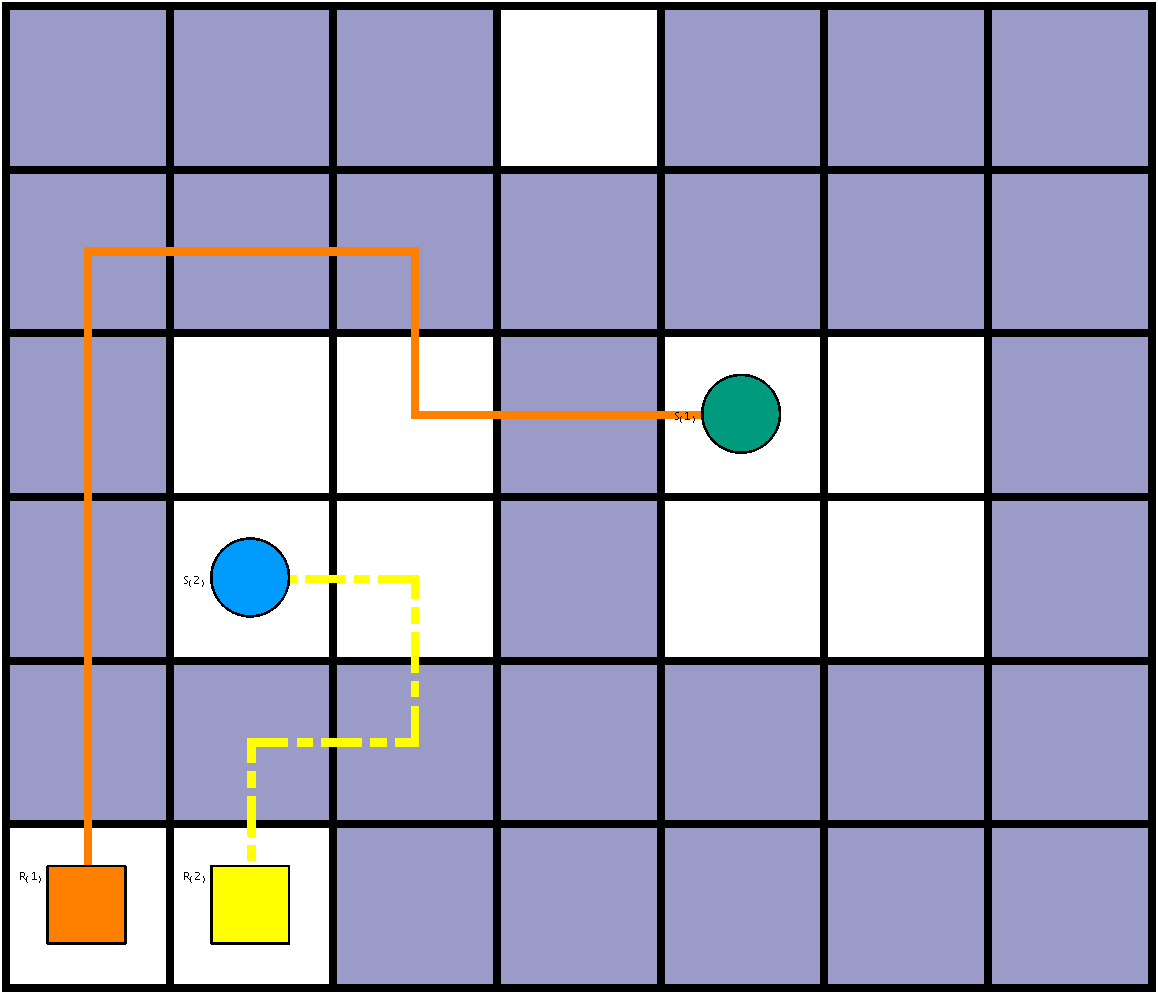
\includegraphics[scale=0.2]{img/asprilo_nc.png}
    \caption{Asprilo visualization for plan from Listing 16 without constraint.}
\end{subfigure}%
\hspace{10px}
\begin{subfigure}{.45\textwidth}
    \centering
    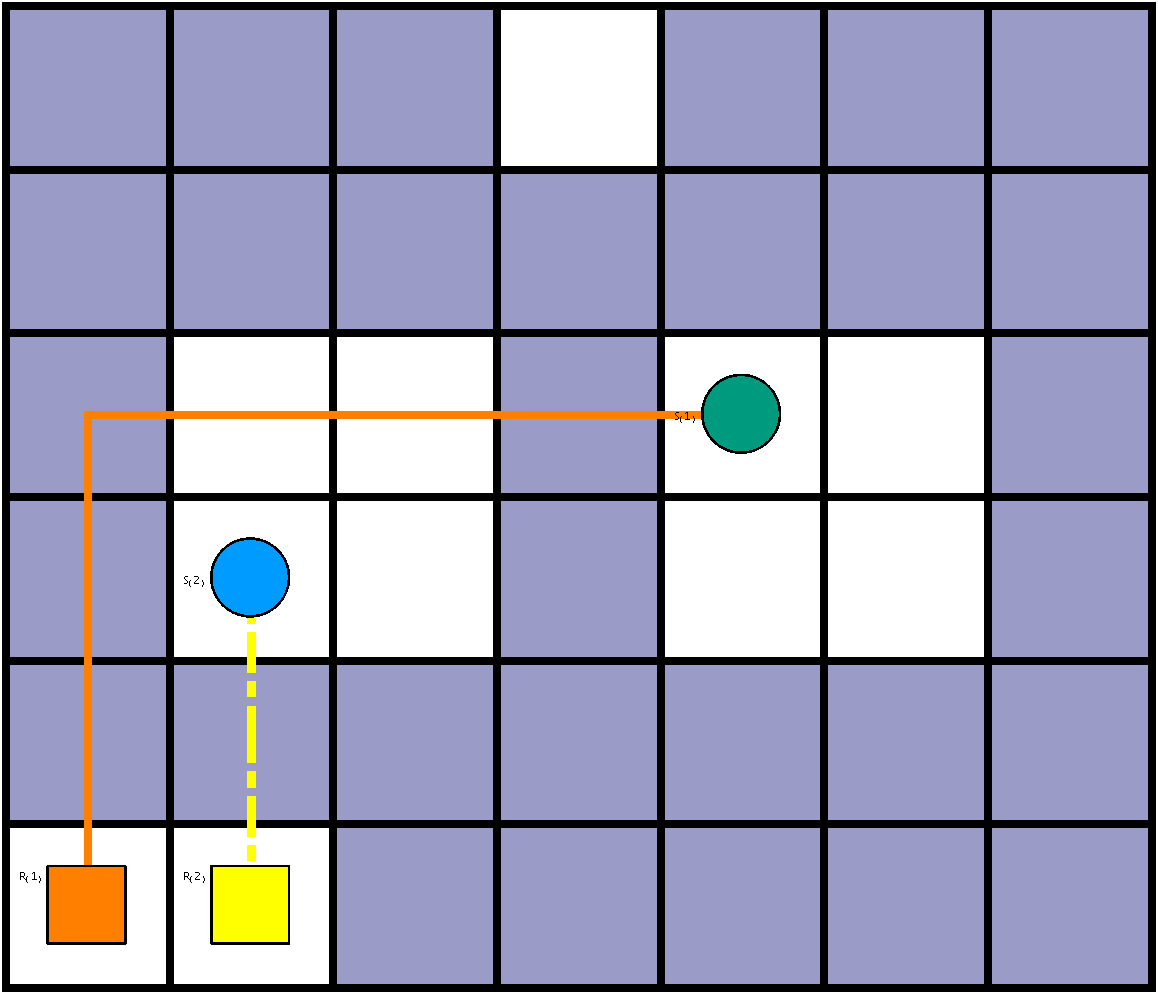
\includegraphics[scale=0.2]{img/asprilo_ur.png}
    \caption{Asprilo visualization for plan following constraint of Listing 17.}
\end{subfigure}
\caption{Images from $\asprilo$'s visualizer corresponding to presented plans. Robots are represented by squares and destinations by circles.}
\end{figure}


The constraint in Listing 17 removes any plan in which the temporal formula is not satisfied. In this case the formula corresponds to $\Next (\mathit{move(robot(R),UP)} \until (\mathit{move(robot(R),RIGHT)} \until \alwaysF \mathit{wait(robot(R))}))$, restricting plans to start with moves up followed by moves right and then waiting. The next operator $\Next$ is necessary at the beginning, since movements in $\asprilo$ start at time point 1. As we can notice, this constraint includes in its body the domain specific predicates \texttt{robot/1}, \texttt{right/1} and \texttt{up/1}.
To address the need of this predicates during the translation the instance is incorporated in the call to $\gringo$ as shown in the workflow overview\footnote{In this case we also require the inclusion of the initialization rules in Listing 14(1-9), as well as the auxiliary predicates for directions.}. 
Consequently, the call to the grounder instantiates the variables yielding one constraint for each robot. Then, the translation deals with the multiple constraints by generating several corresponding initial states of the automaton which are treated as independent automata. 


In the previous section we explained how the automata encoding assumes that all propositions included in the temporal/dynamic formula appear in predicate \texttt{in\_trace\_at/2} with their corresponding identifier from the reification process. 
Therefore, the plans generated by $\asprilo$, such as the one in Listing 15, need to be linked to the identifiers used in \texttt{in\_trace\_at/2}. To achieve such behavior, we construct the additional predicate \texttt{id\_map/2} during the translation of the automata. In this predicate, we gather the linearized abstract syntax tree from gringo into a tuple for a more readable mapping of identifiers. Using this predicate, we write the encoding, which we call `glue', linking all the domain-specific predicates used in the temporal constraint with \texttt{in\_trace\_at/2}. 

\begin{center}
    \begin{lstlisting}[] 
in_trace_at(I,T) :- 
    move(robot(R),(X,Y),T), 
    id_map(I,("move",("robot",N),(X,Y))).

in_trace_at(I,T) :- 
    wait(robot(R),(X,Y),T), 
    id_map(I,("wait",("robot",N))).
    \end{lstlisting}
\captionof{lstlisting}{Glue encoding for movement and position predicates in $\asprilo$.}
\end{center}

The `glue' encoding is then passed to the last call to $\clingo$ along with the instance and planning encoding. Even though the requirement of such an ad-hoc construction could be avoided by using an external script, we opted for an implementation using only ASP. Thus, this additional encoding must be included to complete the integration of any application to our approach.
